\documentclass{beamer}
 \usepackage{beamerthemedefault, multimedia}
 \useoutertheme{smoothbars}
 \useinnertheme[shadow=true]{rounded}
 \setbeamercovered{transparent}
 \setbeamertemplate{navigation symbols}{}
 \setbeamertemplate{footline}[frame number]
\usepackage{graphicx}
\usepackage{morefloats}
\usepackage{amsmath}
\usepackage{amssymb}
\usepackage{rotating}
%\graphicspath{{../../experiments/timbralSimilaritySol/report/tex/}{figures/}{tex/}{../figures/}{../../}{../}}
\title{Scattering for similarity search of playing technique}
\author{ Mathieu Lagrange }

\begin{document}

\maketitle

\begin{frame}\frametitle{Context}
  \begin{itemize}
    \item Technical need: explore a database of recordings of musical instrument playing techniques using computational similarity and automatic ranking techniques
    \item Representing of musical sound signals mostly focus on the frequency distribution of energy
    \item For playing techniques, this is probably not sufficient due to intensive use of modulations
    \item Aim: have a representation that is expressive enough to flexicably adapt to different aspects of musical instrument perception
  \end{itemize}
\end{frame}

\begin{frame}\frametitle{Data}
\begin{itemize}
  \item audio recordings of individual tones of:
  \item instruments, with appendums
  \item playing techniques
  \item nuances
  \item pitch
\end{itemize}
\end{frame}

\begin{frame}\frametitle{Numbers}
\begin{itemize}
  \item number of items is large: > 10 000
  \item number of classes is medium: < 200
  \item number of dimensions too: < 1000
\end{itemize}
\end{frame}

\begin{frame}\frametitle{Processing steps}
\begin{itemize}
  \item features: mel, mfccs, time / frequency wavelet scattering
  \item projection: linear discriminant analysis (lda), large margin nearest neighbors (lmnn)
  \item metric: precision @ 5 (p@5)
\end{itemize}
\end{frame}

\begin{frame}\frametitle{Features}
\begin{itemize}
  \item mel: spectral features on log frequency scale
  \item mfccs: mel projected on a DCT basis
  \item time / frequency wavelet scattering
\end{itemize}
\end{frame}

\begin{frame}\frametitle{Projection}
\begin{itemize}
  \item lda: projection in a (C-1) dimensional space that best separate the classes
  \item lmnn: malahanobis distance metric with projection matrix optimized to achieve best p@k on the training dataset
\end{itemize}
\url{http://jmlr.csail.mit.edu/papers/volume10/weinberger09a/weinberger09a.pdf}
\end{frame}

\begin{frame}\frametitle{Metric}
\begin{itemize}
  \item the precision @ k is a ranking metric
  \item it counts the number of items closest to a query item of the same class than the query item
\end{itemize}
\end{frame}

\begin{frame}\frametitle{Agenda}
\begin{itemize}
  \item experimental design
  \item dataset
  \item features
  \item projection technique
  \item control potential overfit of learnt projection with randomization and dimensionality expansion
  \item control potential overfit of learnt projection with dataset splitting
  \item study the impact of the observation window size
\end{itemize}
\end{frame}

\begin{frame}\frametitle{Factors flow graph}
\begin{center}
\begin{figure}
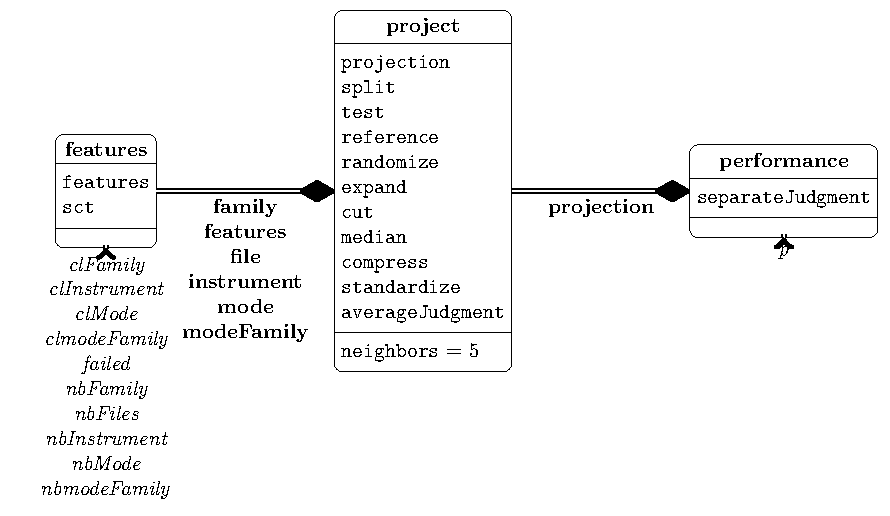
\includegraphics[width=\textwidth,height=0.8\textheight,keepaspectratio]{./figures/factors.pdf}
\label{factorFlowGraph}
\end{figure}
\end{center}
\end{frame}

\begin{frame}\frametitle{Sol db}

\begin{table}
\begin{center}
\
\setlength{\tabcolsep}{.16667em}
\begin{tabular}{cc}
nbFiles & 25444 \\
\hline
nbFamily & 16 \\
nbInstrument & 33 \\
nbMode & 469 \\
nbmodeFamily & 143 \\
\end{tabular}
\end{center}
\label{fenuSc25}
\end{table}

\end{frame}
\begin{frame}\frametitle{Sol db}

\begin{table}
\begin{center}
\
\setlength{\tabcolsep}{.16667em}
\begin{tabular}{cc}
clFamily & 1590 $\pm$936 \\
\hline
clInstrument & 771 $\pm$814 \\
clMode & 54 $\pm$59 \\
clmodeFamily & 178 $\pm$429 \\
\end{tabular}
\end{center}
\label{fenuSc25}
\end{table}

\end{frame}
\begin{frame}\frametitle{Mel / mfcc: sct: 25, projection: none, split: none, reference: family, randomize: 0, expand: 0}

\begin{table}
\begin{center}
\
\setlength{\tabcolsep}{.16667em}
\begin{tabular}{lllc}
features & cut & standardize & p (\%) \\
\hline
mfcc & 0 & 0 & 85 \\
mfcc & 0 & 1 & 84 \\
mfcc & 1 & 0 & 88 \\
mfcc & 1 & 1 & \textbf{\textcolor{red}{89}} \\
mel &  & 0 & 53 \\
mel &  & 1 & 50 \\
\end{tabular}
\end{center}
\label{sc25PrnoSpnoRefaRa0Ex0}
\end{table}

\end{frame}
\begin{frame}\frametitle{Mel / mfcc: sct: 25, projection: none, split: none, reference: modeFamily, randomize: 0, expand: 0}

\begin{table}
\begin{center}
\
\setlength{\tabcolsep}{.16667em}
\begin{tabular}{lllc}
features & cut & standardize & p (\%) \\
\hline
mfcc & 0 & 0 & 35 \\
mfcc & 0 & 1 & 32 \\
mfcc & 1 & 0 & \textbf{\textcolor{red}{46}} \\
mfcc & 1 & 1 & 45 \\
mel &  & 0 & 19 \\
mel &  & 1 & 19 \\
\end{tabular}
\end{center}
\label{sc25PrnoSpnoRemofaRa0Ex0}
\end{table}

\end{frame}
\begin{frame}\frametitle{Scattering: features: scat, sct: 25, projection: none, split: none, reference: family, randomize: 0}

\begin{table}
\begin{center}
\
\setlength{\tabcolsep}{.16667em}
\begin{tabular}{lllc}
median & compress & standardize & p (\%) \\
\hline
0 & 0 & 0 & 64 \\
0 & 0 & 1 & 76 \\
0 & 1 & 0 & 84 \\
0 & 1 & 1 & 83 \\
1 & 0 & 0 & 77 \\
1 & 0 & 1 & 76 \\
1 & 1 & 0 & \textbf{\textcolor{red}{89}} \\
1 & 1 & 1 & 89 \\
\end{tabular}
\end{center}
\label{fescSc25PrnoSpnoRefaRa0}
\end{table}

\end{frame}
\begin{frame}\frametitle{Scattering: features: scat, sct: 25, projection: none, split: none, reference: modeFamily, randomize: 0}

\begin{table}
\begin{center}
\
\setlength{\tabcolsep}{.16667em}
\begin{tabular}{lllc}
median & compress & standardize & p (\%) \\
\hline
0 & 0 & 0 & 28 \\
0 & 0 & 1 & 38 \\
0 & 1 & 0 & 43 \\
0 & 1 & 1 & 43 \\
1 & 0 & 0 & 40 \\
1 & 0 & 1 & 38 \\
1 & 1 & 0 & 50 \\
1 & 1 & 1 & \textbf{\textcolor{red}{50}} \\
\end{tabular}
\end{center}
\label{fescSc25PrnoSpnoRemofaRa0}
\end{table}

\end{frame}
\begin{frame}\frametitle{Projection: sct: 25, split: none, reference: family, randomize: 0, expand: 0, cut: 1, median: 1, compress: 1, standardize: 1}

\begin{table}
\begin{center}
\
\setlength{\tabcolsep}{.16667em}
\begin{tabular}{lcc}
features & mfcc & scat \\
\hline
none & 89 & 89 \\
lmnn & 90 & 98 \\
lda & 87 & 96 \\
\end{tabular}
\end{center}
\label{sc25SpnoRefaRa0Ex0Cu1Me1Co1St1}
\end{table}

\end{frame}
\begin{frame}\frametitle{Projection: sct: 25, split: none, reference: modeFamily, randomize: 0, expand: 0, cut: 1, median: 1, compress: 1, standardize: 1}

\begin{table}
\begin{center}
\
\setlength{\tabcolsep}{.16667em}
\begin{tabular}{lcc}
features & mfcc & scat \\
\hline
none & 45 & 50 \\
lmnn & 48 & 53 \\
lda & 50 & 52 \\
\end{tabular}
\end{center}
\label{sc25SpnoRemofaRa0Ex0Cu1Me1Co1St1}
\end{table}

\end{frame}
\begin{frame}\frametitle{Control learning: sct: 25, split: none, reference: family, cut: 1, median: 1, compress: 1, standardize: 1}

\begin{table}
\begin{center}
\
\setlength{\tabcolsep}{.16667em}
\begin{tabular}{lllccc}
features & randomize & expand & none & lmnn & lda \\
\hline
mfcc & 0 &    0 & 89 & 90 & 87 \\
mfcc & 0 &  494 & 88 & 91 & 89 \\
mfcc & 1 &    0 &  8 &  8 &  8 \\
mfcc & 1 &  494 &  8 &  9 &  9 \\
scat & 0 &  & 89 & 98 & 96 \\
scat & 1 &  &  8 &  9 &  9 \\
\end{tabular}
\end{center}
\label{sc25SpnoRefaCu1Me1Co1St1}
\end{table}

\end{frame}
\begin{frame}\frametitle{Control learning: sct: 25, split: none, reference: modeFamily, cut: 1, median: 1, compress: 1, standardize: 1}

\begin{table}
\begin{center}
\
\setlength{\tabcolsep}{.16667em}
\begin{tabular}{lllccc}
features & randomize & expand & none & lmnn & lda \\
\hline
mfcc & 0 &    0 & 45 & 48 & 50 \\
mfcc & 0 &  494 & 43 & 49 & 49 \\
mfcc & 1 &    0 &  5 &  5 &  5 \\
mfcc & 1 &  494 &  5 &  4 &  5 \\
scat & 0 &  & 50 & 53 & 52 \\
scat & 1 &  &  5 &  4 &  5 \\
\end{tabular}
\end{center}
\label{sc25SpnoRemofaCu1Me1Co1St1}
\end{table}

\end{frame}

\clearpage


\begin{frame}\frametitle{\small db splitting: sct: 25, test: 1, reference: family, randomize: 0, expand: 0, cut: 1, median: 1, compress: 1, standardize: 1}
\begin{center}
\begin{figure}
\centering
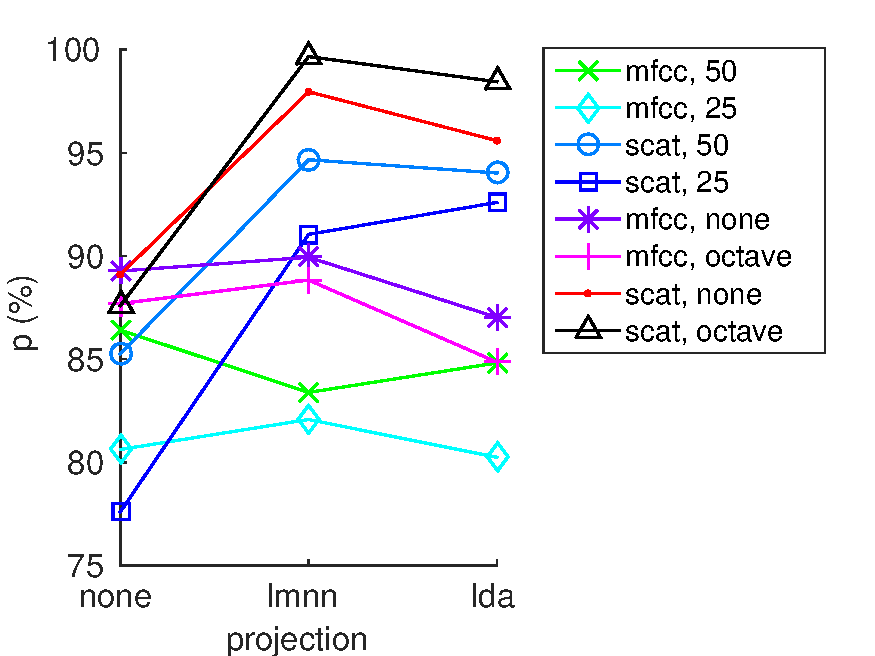
\includegraphics[width=\textwidth,height=0.8\textheight,keepaspectratio]{./figures/Fig141.pdf}
\label{sc25Te1RefaRa0Ex0Cu1Me1Co1St1}
\end{figure}
\end{center}


\end{frame}

\begin{frame}\frametitle{\small db splitting: sct: 25, test: 1, reference: modeFamily, randomize: 0, expand: 0, cut: 1, median: 1, compress: 1, standardize: 1}
\begin{center}
\begin{figure}
\centering
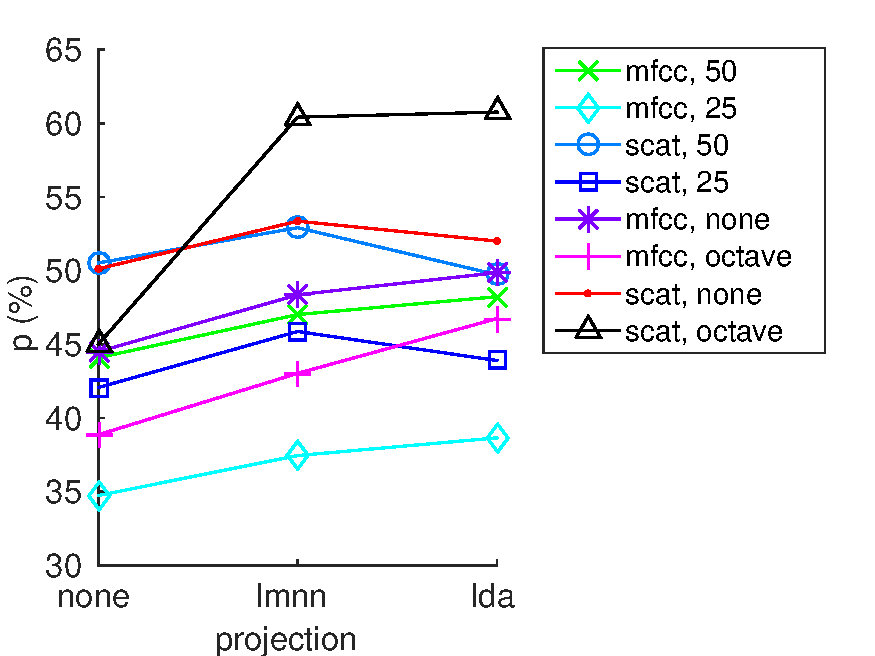
\includegraphics[width=\textwidth,height=0.8\textheight,keepaspectratio]{./figures/Fig142.pdf}
\label{sc25Te1RemofaRa0Ex0Cu1Me1Co1St1}
\end{figure}
\end{center}


\end{frame}

\begin{frame}\frametitle{\small T: features: mfcc, reference: family, split: none, randomize: 0, expand: 0, cut: 1, standardize: 1}
\begin{center}
\begin{figure}
\centering
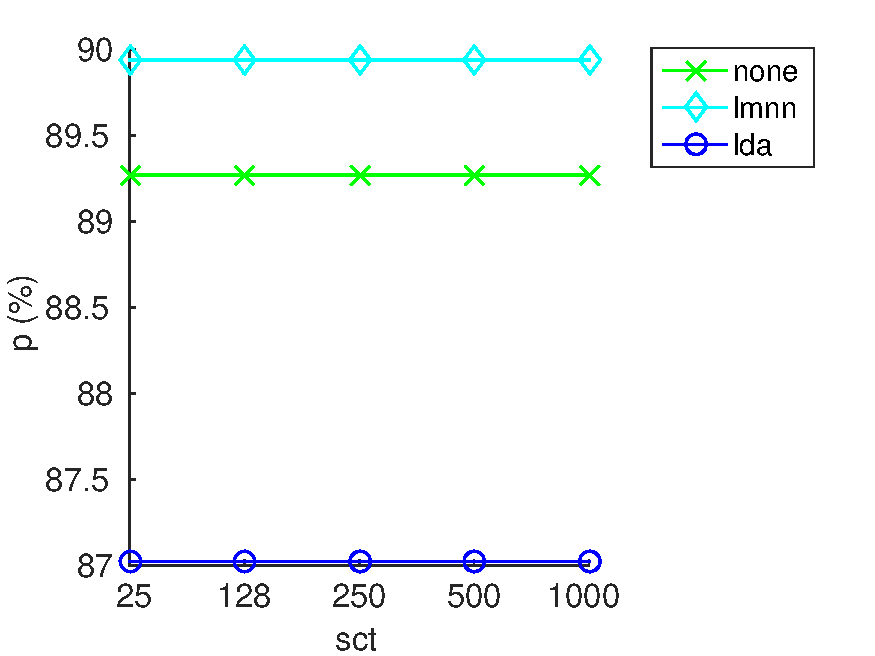
\includegraphics[width=\textwidth,height=0.8\textheight,keepaspectratio]{./figures/Fig143.pdf}
\label{femfRefaSpnoRa0Ex0Cu1St1}
\end{figure}
\end{center}


\end{frame}

\begin{frame}\frametitle{\small T: features: scat, reference: family, split: none, randomize: 0, median: 1, compress: 1, standardize: 1}
\begin{center}
\begin{figure}
\centering
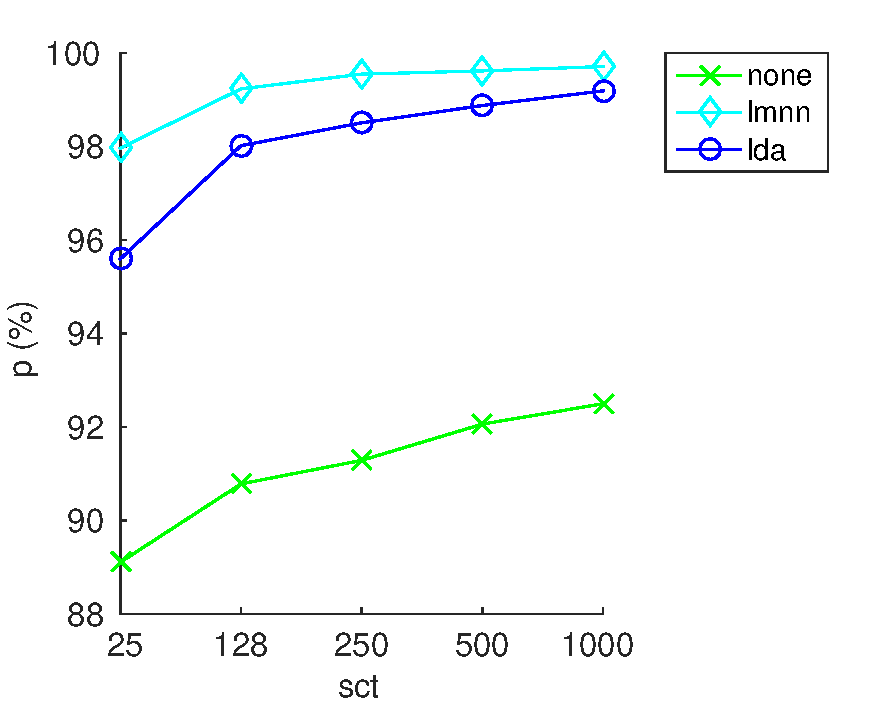
\includegraphics[width=\textwidth,height=0.8\textheight,keepaspectratio]{./figures/Fig144.pdf}
\label{fescRefaSpnoRa0Me1Co1St1}
\end{figure}
\end{center}


\end{frame}

\begin{frame}\frametitle{\small T: reference: family, split: none, randomize: 0, expand: 0, cut: 1, median: 1, compress: 1, standardize: 1}
\begin{center}
\begin{figure}
\centering
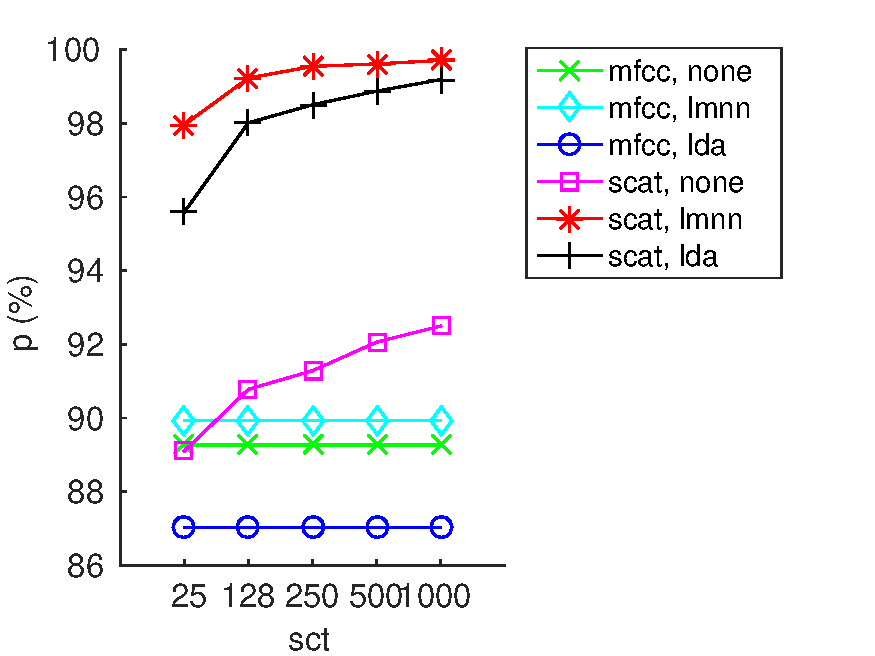
\includegraphics[width=\textwidth,height=0.8\textheight,keepaspectratio]{./figures/Fig145.pdf}
\label{refaSpnoRa0Ex0Cu1Me1Co1St1}
\end{figure}
\end{center}


\end{frame}

\begin{frame}\frametitle{\small T: features: mfcc, reference: modeFamily, split: none, randomize: 0, expand: 0, cut: 1, standardize: 1}
\begin{center}
\begin{figure}
\centering
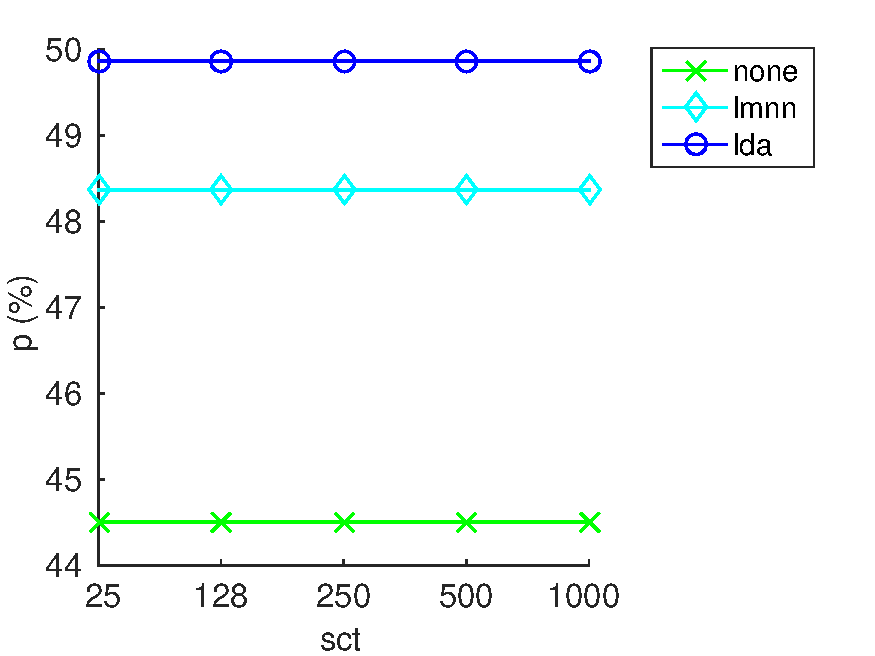
\includegraphics[width=\textwidth,height=0.8\textheight,keepaspectratio]{./figures/Fig146.pdf}
\label{femfRemofaSpnoRa0Ex0Cu1St1}
\end{figure}
\end{center}


\end{frame}

\begin{frame}\frametitle{\small T: features: scat, reference: modeFamily, split: none, randomize: 0, median: 1, compress: 1, standardize: 1}
\begin{center}
\begin{figure}
\centering
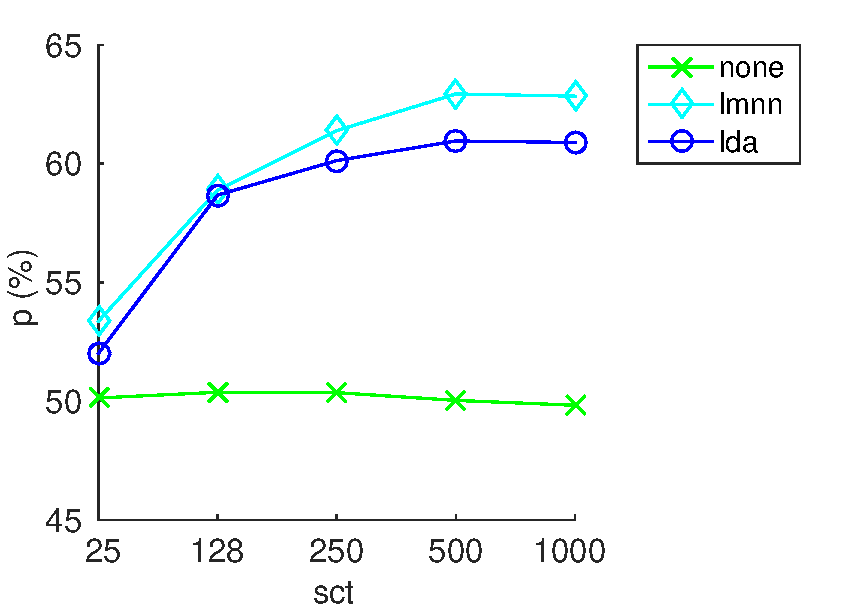
\includegraphics[width=\textwidth,height=0.8\textheight,keepaspectratio]{./figures/Fig147.pdf}
\label{fescRemofaSpnoRa0Me1Co1St1}
\end{figure}
\end{center}


\end{frame}

\begin{frame}\frametitle{\small T: reference: modeFamily, split: none, randomize: 0, expand: 0, cut: 1, median: 1, compress: 1, standardize: 1}
\begin{center}
\begin{figure}
\centering
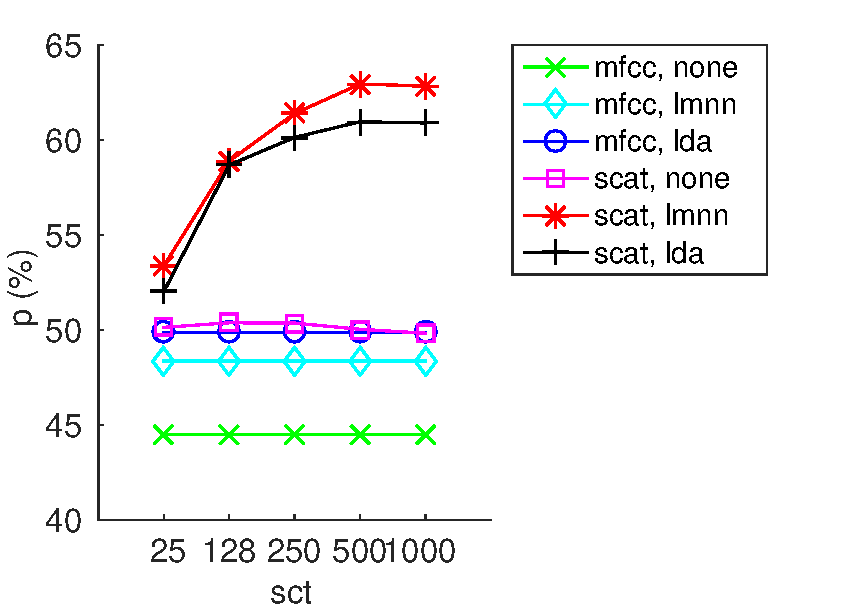
\includegraphics[width=\textwidth,height=0.8\textheight,keepaspectratio]{./figures/Fig148.pdf}
\label{remofaSpnoRa0Ex0Cu1Me1Co1St1}
\end{figure}
\end{center}


\end{frame}

\begin{frame}\frametitle{\small conclusion: split: none, randomize: 0, expand: 0, cut: 1, median: 1, compress: 1, standardize: 1}
\begin{center}
\begin{figure}
\centering
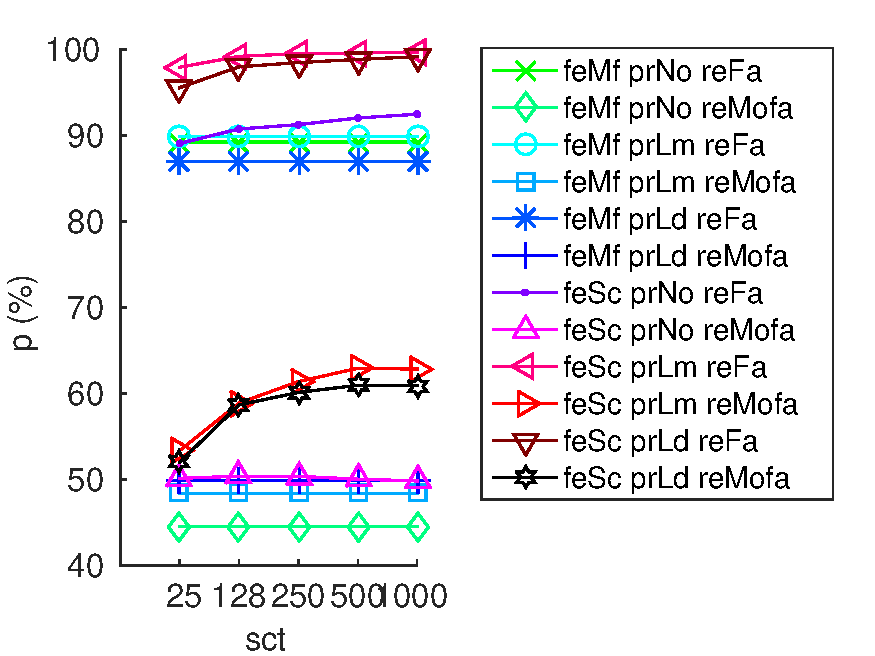
\includegraphics[width=\textwidth,height=0.8\textheight,keepaspectratio]{./figures/Fig149.pdf}
\label{spnoRa0Ex0Cu1Me1Co1St1}
\end{figure}
\end{center}


\end{frame}


\end{document}
